\documentclass[aspectratio=169]{beamer}
\usepackage[utf8]{inputenc}
\usepackage{tikz} % for QR code overlay

% code snippets
\usepackage{minted}
\newmintedfile[dockercode]{dockerfile}{
  % bgcolor=mintedbackground,
  fontfamily=tt,
  linenos=true,
  numberblanklines=true,
  numbersep=5pt,
  gobble=0,
  frame=leftline,
  framerule=0.4pt,
  framesep=2mm,
  funcnamehighlighting=true,
  tabsize=4,
  obeytabs=false,
  mathescape=false
  samepage=false, %with this setting you can force the list to appear on the same page
  showspaces=false,
  showtabs =false,
  texcl=false,
}
\newminted[bashcode]{bash}{
  % bgcolor=mintedbackground,
  fontfamily=tt,
  linenos=true,
  numberblanklines=true,
  numbersep=5pt,
  gobble=0,
  frame=leftline,
  framerule=0.4pt,
  framesep=2mm,
  funcnamehighlighting=true,
  tabsize=4,
  obeytabs=false,
  mathescape=false
  samepage=false, %with this setting you can force the list to appear on the same page
  showspaces=false,
  showtabs =false,
  texcl=false,
}

% biblatex (requires biber; sudo pacman -S biber)
\usepackage[]{biblatex} % biblatex
\addbibresource{./src/bib/fhe.bib}
\addbibresource{./src/bib/dl.bib}
\addbibresource{./src/bib/misc.bib}

\usepackage{graphicx}
\graphicspath{ {./src/img/} }

\usetheme{Boadilla}
\usecolortheme{rose}
% \beamerdefaultoverlayspecification{<+->} % this will turn it into slides

\title{Augmented Agronomist}
\subtitle{Synthesis of Privacy-Preserving Deep Learning and Robotics to Assist Decision Support}
\author{George Onoufriou\\University of Lincoln}
\date{\today}

\begin{document}

\addtobeamertemplate{frametitle}{}{%
\begin{tikzpicture}[remember picture,overlay]
\node[anchor=north east,yshift=2pt] at (current page.north east) {
\includegraphics[height=1.5cm]{qrcode.png}};
\end{tikzpicture}}

  \frame{\titlepage}

% ----- ABOUT ME PAGE
  \begin{frame}
    \frametitle{About}
    \begin{columns}
      \begin{column}{0.5\textwidth}
        Myself:
        \begin{itemize}
          \item PhD Candidate Computer/ Data Science
          \item Privacy and Linux Enthusiast
        \end{itemize}
        Presentation:
        \begin{itemize}
          \item Slides are available via the QR code or link (QR available on every slide)
          \item Submit an issue in repository if seeing this later but still have questions
          \item Broad overview of yield prediction/ neural network techniques
        \end{itemize}
      \end{column}
      \begin{column}{0.5\textwidth}
        \begin{figure}[th!]
          \centering
          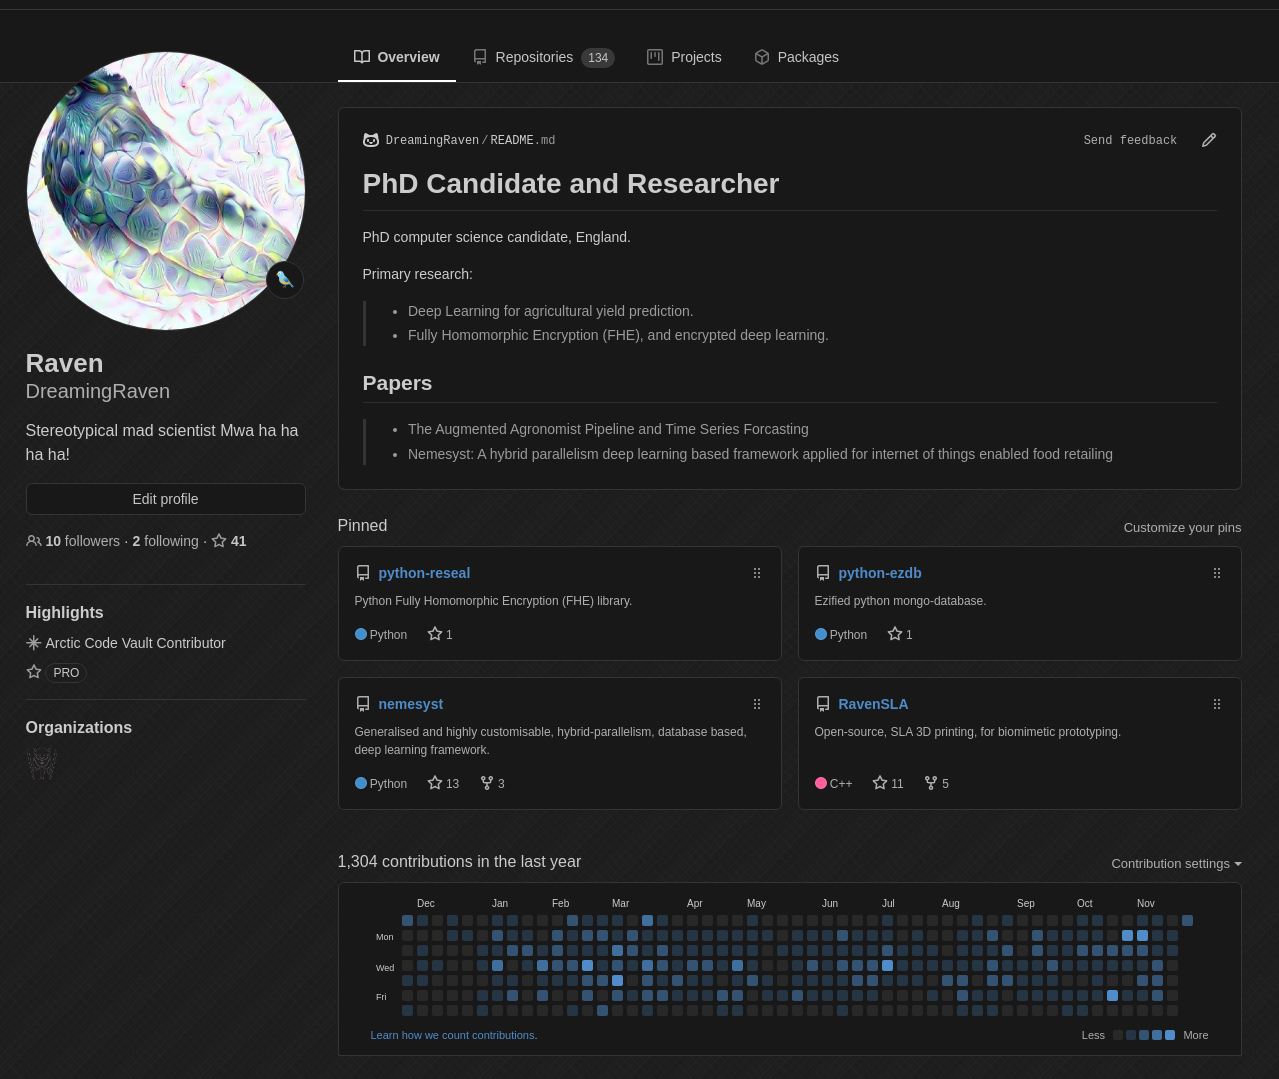
\includegraphics[width=0.8\textwidth]{gh.png}
          \caption{GitHub profile page where you can come to see my work and chat. \autocite{repository}}
          \label{fig:gh}
        \end{figure}
      \end{column}
    \end{columns}
  \end{frame}

% ----- PROBLEM PAGE
  \begin{frame}
    \frametitle{The Agricultural Problem}
    \begin{columns}
      \begin{column}{0.5\textwidth}
        Problem:
        \begin{itemize}
          \item How do you know how much produce any given farm will produce in $x$ weeks time
            \begin{itemize}
              \item 14\%
              \item 50\%
            \end{itemize}
          \item Either
            \begin{itemize}
              \item Have too much (storage, handling, disposal)
              \item Have too little (meeting agreements by importing, competition)
            \end{itemize}
        \end{itemize}
      \end{column}
      \begin{column}{0.5\textwidth}
        \begin{figure}[th!]
          \centering
          \includegraphics[width=0.6\textwidth]{waste.jpg}
          \caption{Waste from early on in the strawberry season starting to pile up. \autocite{repository}}
          \label{fig:gh}
        \end{figure}
      \end{column}
    \end{columns}
  \end{frame}

% ----- YIELD PROBLEM PAGE
  \begin{frame}
    \frametitle{Yield}
    \begin{columns}
      \begin{column}{0.3\textwidth}
        How do you account for:
        \begin{itemize}
          \item High variance between crops, crop locations, and varieties
          \item High variance in behaviour of a single crop over a season
          \item High variance between growers
        \end{itemize}
      \end{column}
      \begin{column}{0.7\textwidth}
        \begin{figure}[th!]
          \centering
          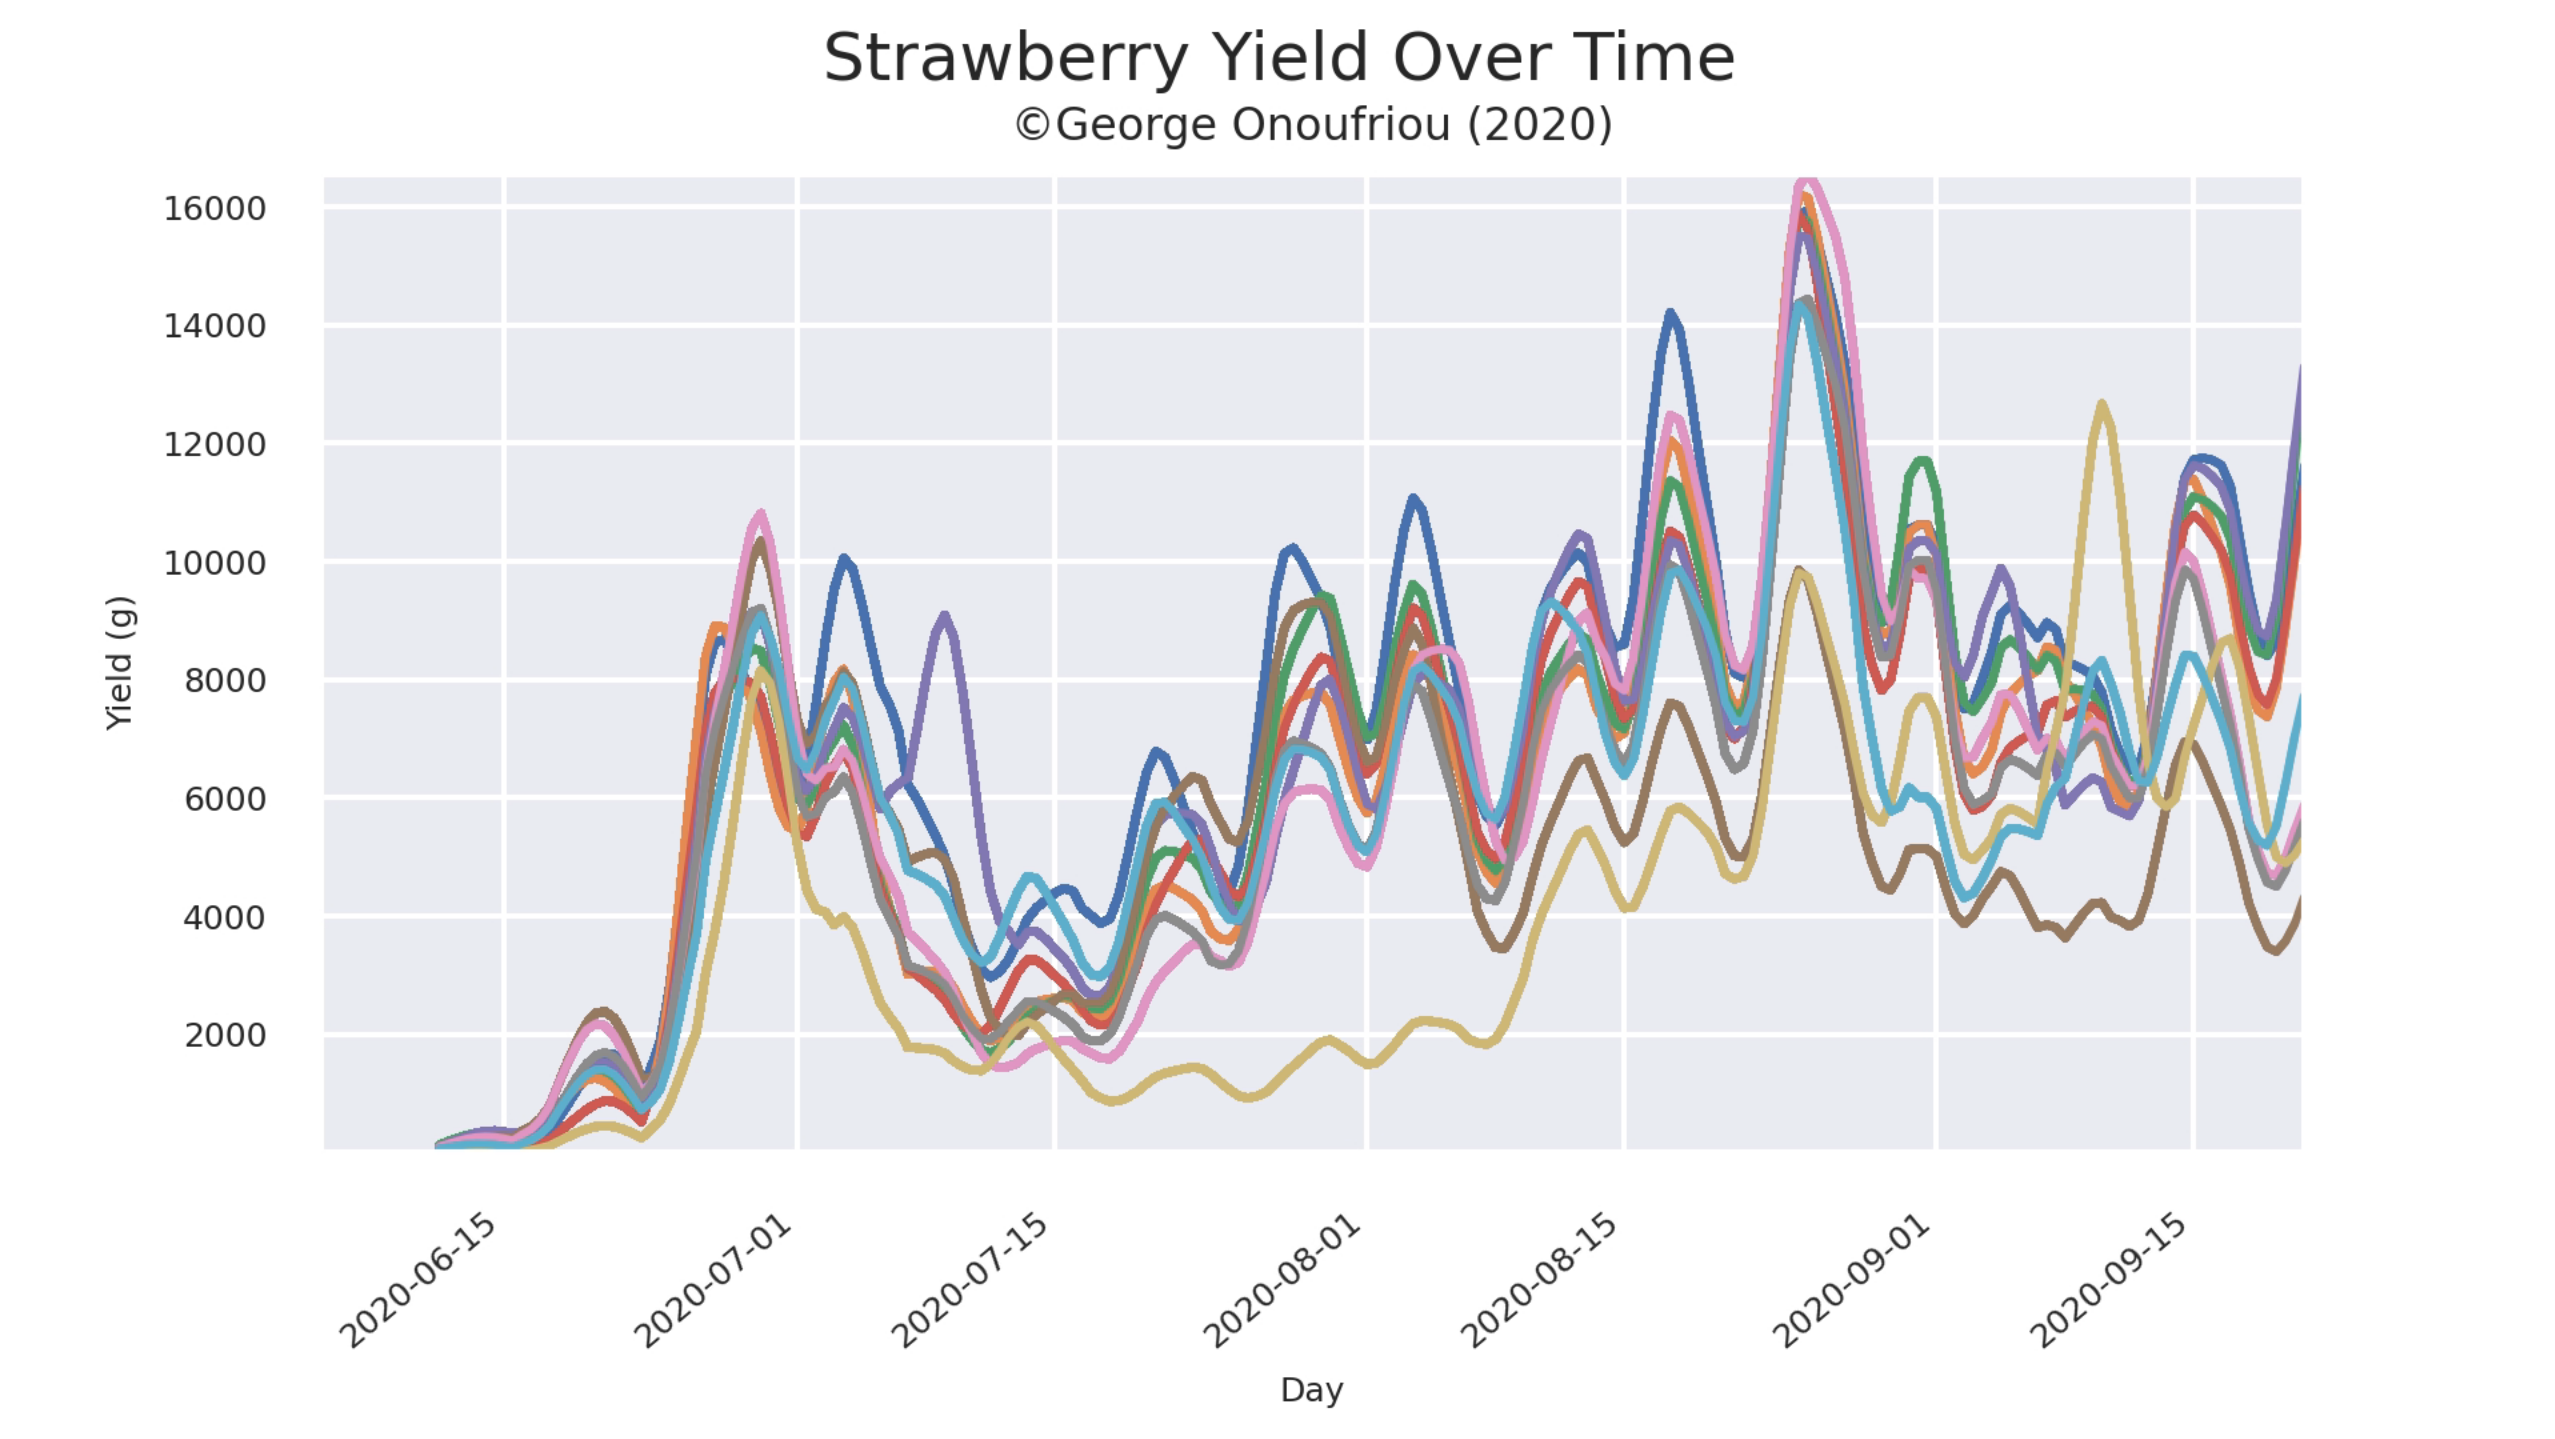
\includegraphics[width=1\textwidth]{yield.png}
          \caption{Yield over a portion of a season example. \autocite{repository}}
          \label{fig:yield}
        \end{figure}
      \end{column}
    \end{columns}
  \end{frame}

% ----- DATA PROBLEM PAGE
  \begin{frame}
    \frametitle{Data}
    \begin{columns}
      \begin{column}{0.5\textwidth}
        What data is valuable:
        \begin{itemize}
          \item Spacial; positions, images of plant and environment, movement, growth. (less common)
          \item Temporal; light, temperature, humidity, precipitation, irrigation, nutrition, wind-speed, etc. (common)
        \end{itemize}
        How readily available is this data:
        \begin{itemize}
          \item expensive equipment
          \item sensitivity to the data, e.g trade-secrets
          \item difficulty to obtaining and sharing
        \end{itemize}
      \end{column}
      \begin{column}{0.5\textwidth}
        \begin{figure}[th!]
          \centering
          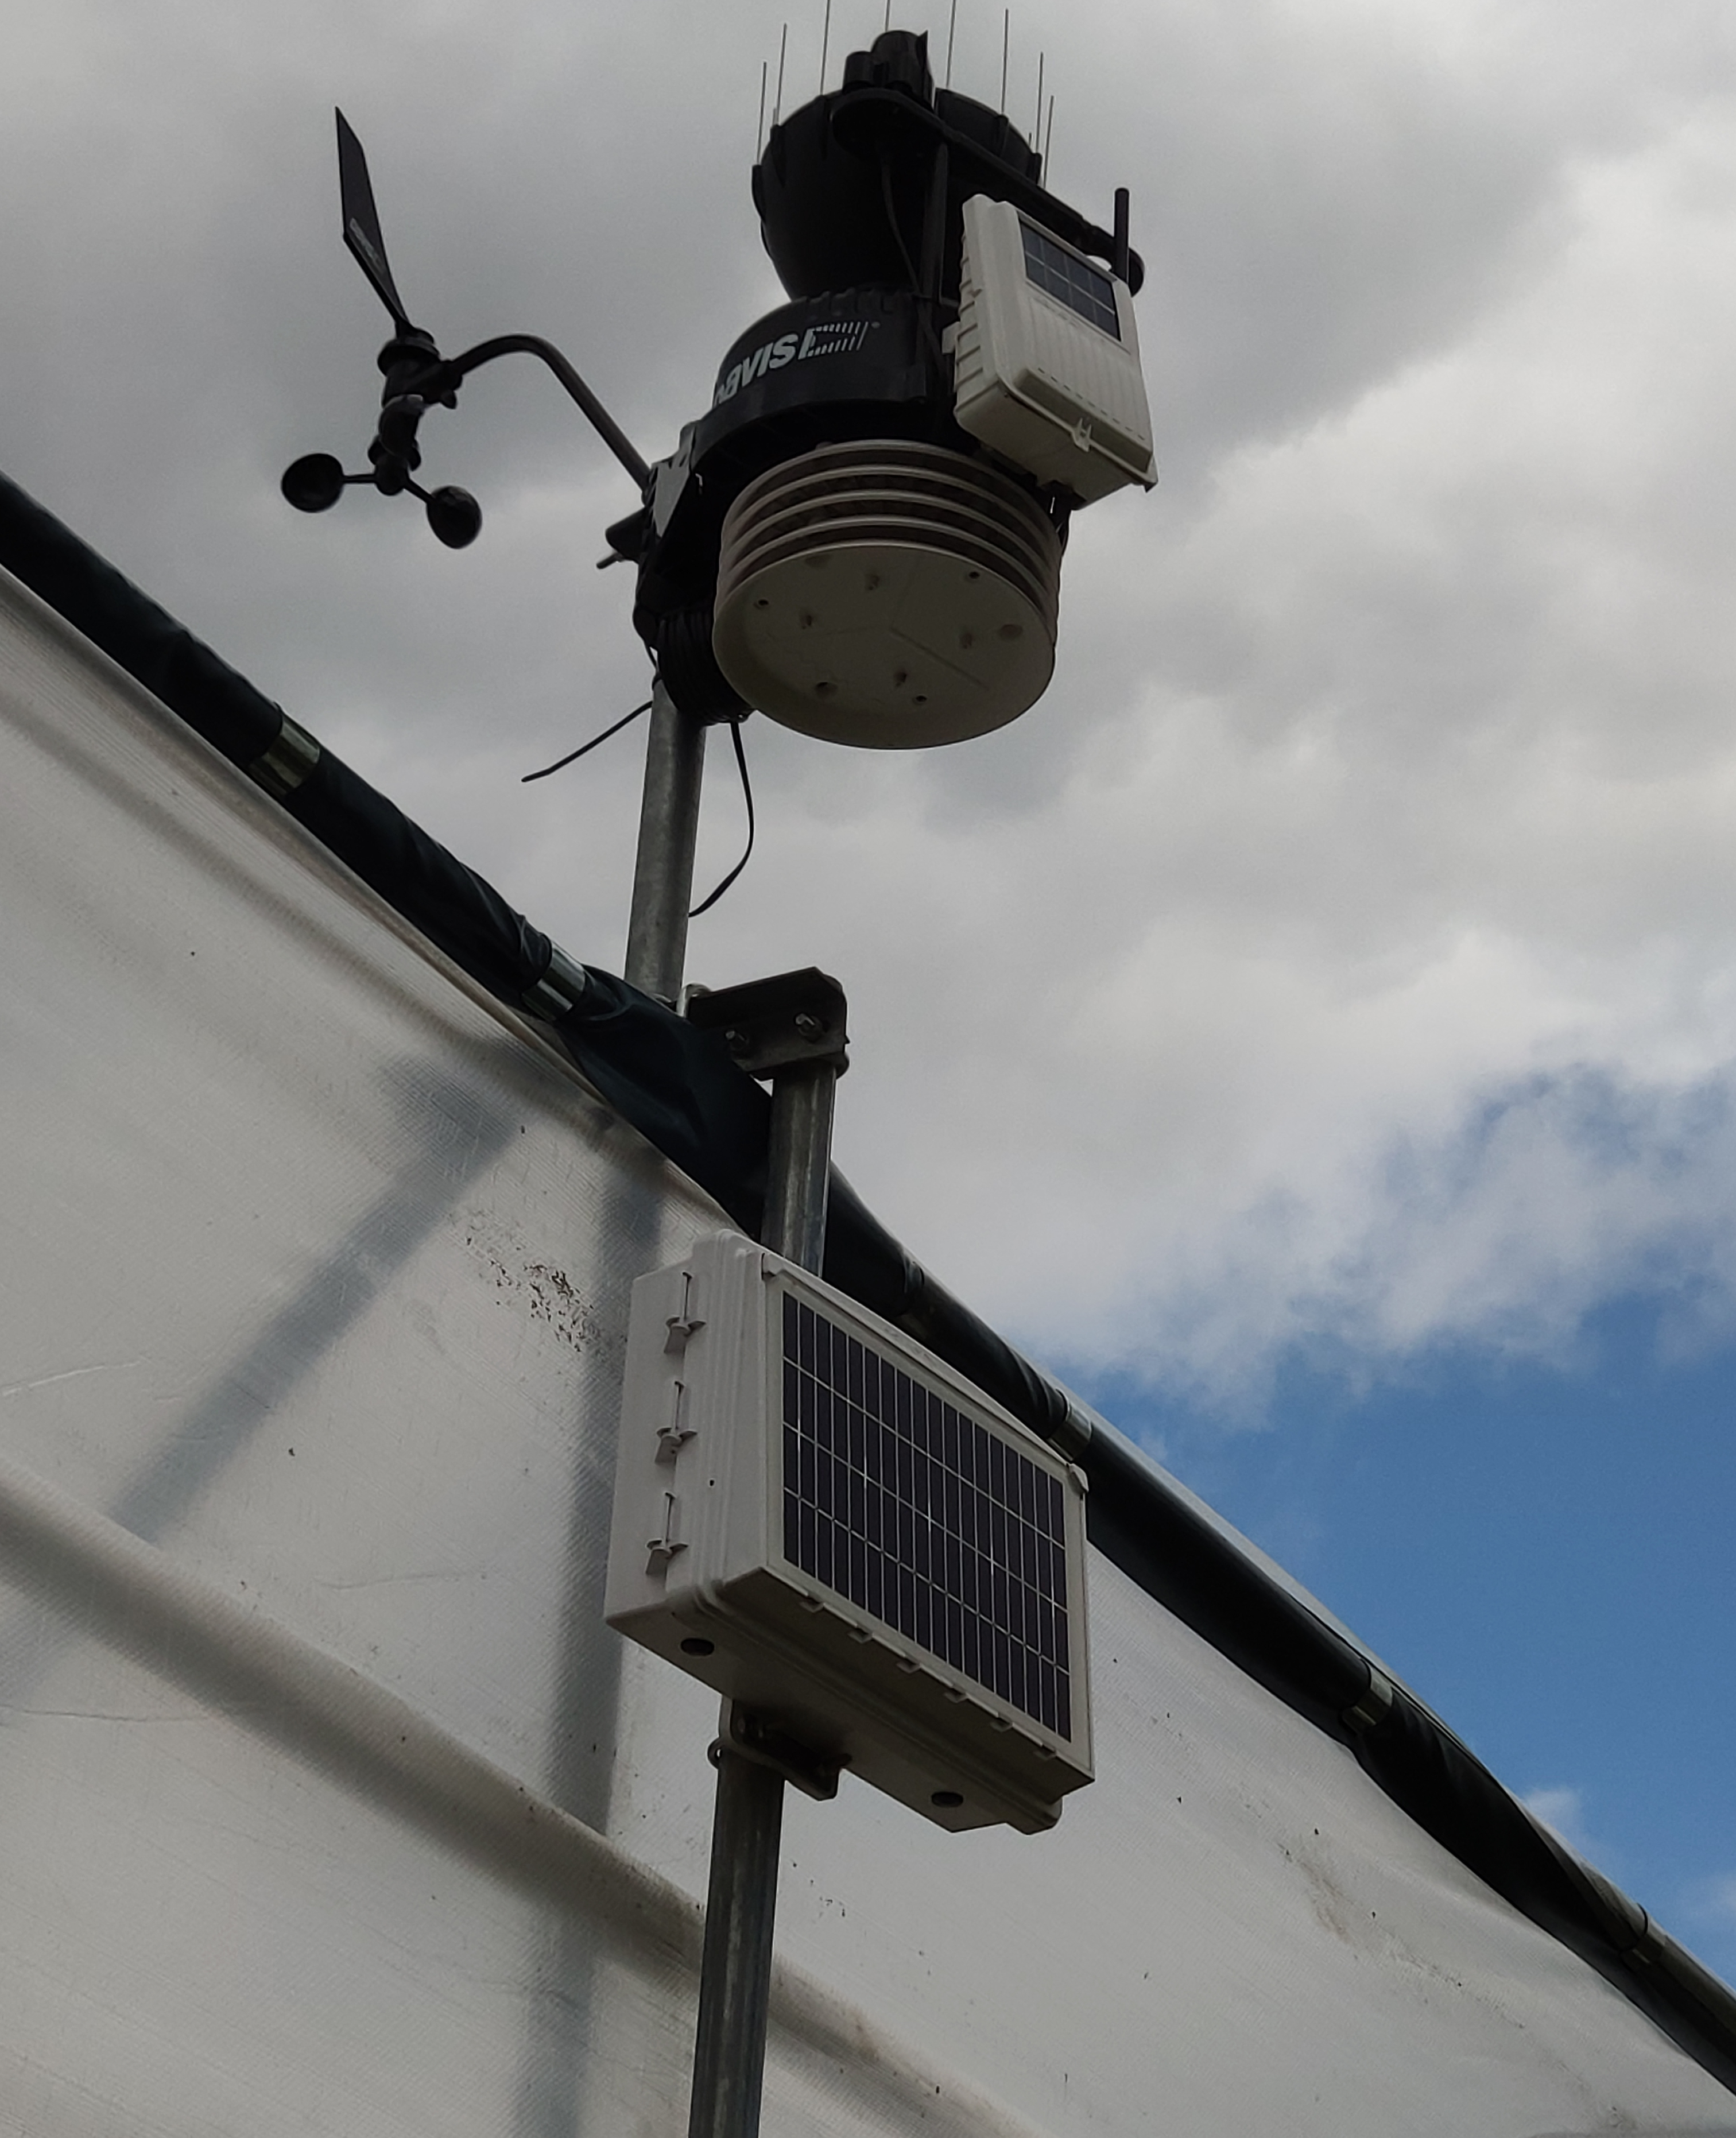
\includegraphics[width=0.55\textwidth]{weather.jpg}
          \caption{Weathervane collecting environmental data in regular intervals. \autocite{repository}}
          \label{fig:yield}
        \end{figure}
      \end{column}
    \end{columns}
  \end{frame}

% ----- MY WORK PAGE
  \begin{frame}
    \frametitle{My Work}
    \begin{columns}
      \begin{column}{0.5\textwidth}
        I work with:
        \begin{itemize}
          \item Deep Learning (subfield of Artificial Intelligence, and probably the coolest part of AI)
          \item Fully Homomorphic Encryption
        \end{itemize}
        Applied to:
        \begin{itemize}
          \item Agriculture; Predicting plant yield, in particular strawberries.
        \end{itemize}
        Further:
        \begin{itemize}
          \item Turning FHE into an open-source encrypted deep learning as a service (EDLaaS) to provide as a business.
        \end{itemize}
      \end{column}
      \begin{column}{0.5\textwidth}
        \begin{figure}[th!]
          \centering
          \includegraphics[angle=-90,origin=c,width=0.55\textwidth]{wasp.jpg}
          \caption{Strawberry tabletop with a wasp having some lunch. \autocite{repository}}
          \label{fig:wasp}
        \end{figure}
      \end{column}
    \end{columns}
  \end{frame}

% ----- REFERENCES PAGE
  \begin{frame}[allowframebreaks]
    \frametitle{References}
    % % biblatex version
    \printbibliography
  \end{frame}

\end{document}
